\chapter{Scenes}
The scenes with images are described below. The squares in the images are particles, white lines are forces and green lines are constraints.

\section{Simple particle scene}
This is a simple particle system. It shows different constraints, like a circular wire constraint and a rod constraint. Besides that it shows gravity force and spring forces. (see figure \ref{fig:Particle})
\begin{figure}[htb!]
    \centering
    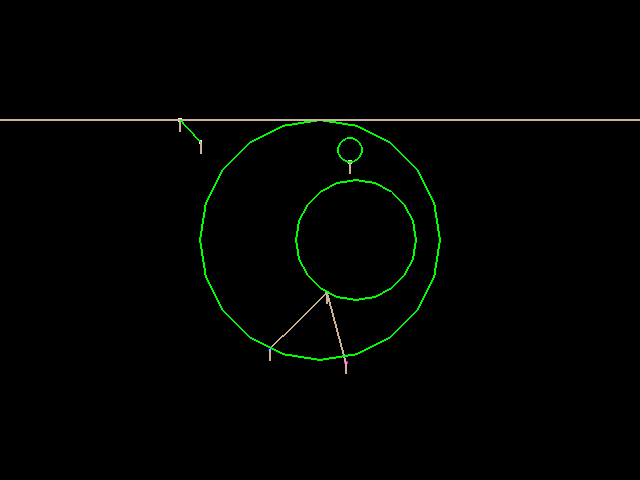
\includegraphics[width=0.6\textwidth]{images/Particle}
    \caption{Particle scene}
    \label{fig:Particle}
\end{figure}

\section{Cloth scene}

The cloth scene in figure \ref{fig:Cloth} is it's initial state. The constraints and springs are on top of each other. We used 2 rod constraints to create a constraint that can be smaller, but not bigger than a certain length.

\begin{figure}[htb!]
    \centering
    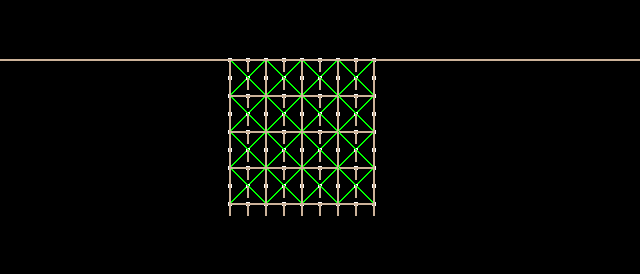
\includegraphics[width=0.8\textwidth]{images/Cloth}
    \caption{The cloth scene}
    \label{fig:Cloth}
\end{figure}


\section{Hair scene}

In figure \ref{fig:HairInit} is the initial hair system shown. between every 3 points there are 2 rod constraints, to create a maximum hair size. On the last edge in the triangle there is a spring force added, to give the hair a curly characteristic. In figure \ref{fig:Hair} it shows how the hair looks like when it is pulled out.

\begin{figure}[htb!]
    \centering
    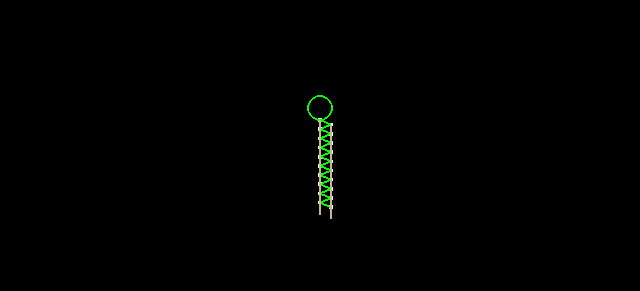
\includegraphics[width=0.8\textwidth]{images/HairInit}
    \caption{The initial hair scene}
    \label{fig:HairInit}
\end{figure}
\begin{figure}[htb!]
    \centering
    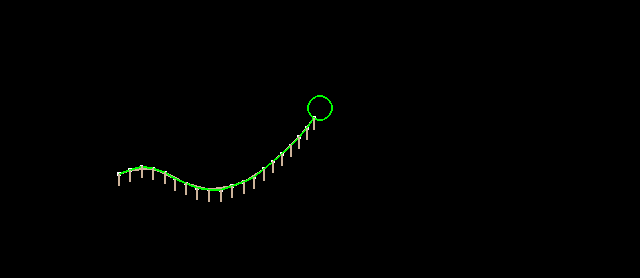
\includegraphics[width=0.8\textwidth]{images/Hair}
    \caption{When the hair is stretched}
    \label{fig:Hair}
\end{figure}

\section{Solar system scene}

Figure \ref{fig:Solar} shows a simple solar system, this shows the point gravity force. These forces are shown in white.

\begin{figure}[htb!]
    \centering
    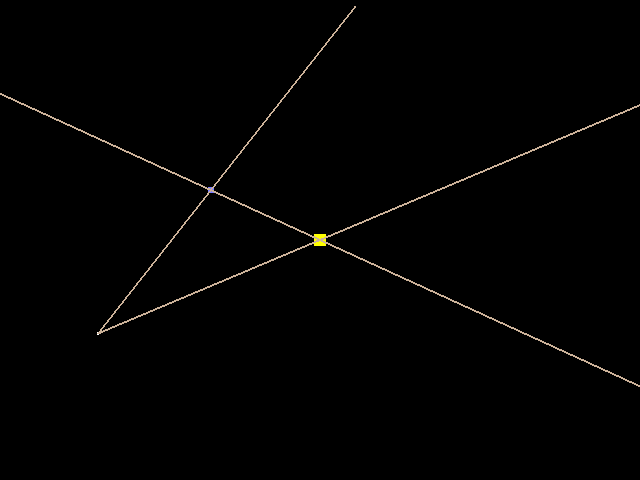
\includegraphics[width=0.6\textwidth]{images/Solar}
    \caption{A simple solar system with 1 sun and 2 celestial body's}
    \label{fig:Solar}
\end{figure}

